\scanpage{17}
\mspage{14}

\figure{
\begin{tikzpicture}\draw[gray] (-.26,.16) .. controls (.27,-.06) and (.13,-.36) .. (-.01,-.28) .. controls (-.17,-.10) and (.18,-.02) .. (.31,.23);\end{tikzpicture}}

La notion de ``morphisme de Dérivateurs'' ``est claire'', c'est un morphisme entre \deleted{des} 2 foncteurs stricts

\[
\mathrm{Diag}^{\unsure{\circ|o}}\longrightarrow\mathrm{Cat}
\]

Donc

\[
u:\mathbb D\unsure{-|\longrightarrow}\mathbb D'
\]

est défini par la donnée, pour \unsure{tt|tout} $I\in\mathrm{Diag}$, de

\[
u_{I}:\mathbb D(I)\to\mathbb D^{\unsure{\prime}}(I)
\]

avec commutativité (stricte ?) pour $f:I\unsure{-|\to}J$

\diagram{\begin{tikzcd}[ampersand replacement=\&]
(1)\& \mathbb D(J)\arrow[r,"{f^{*}_{\mathbb D}}",dash]\arrow[d,"{u_{J}}"'] \& \mathbb D(I)\arrow[d,"{u_{I}}"]\\
\& \mathbb D'(J)\arrow[r,"{f^{*}_{\mathbb D'}}",dash] \& \mathbb D'(I)\, .
\end{tikzcd}}

On a

\diagram{\begin{tikzcd}[ampersand replacement=\&]
(2)\& \underline{\mathrm{Hom}}\,(I,J)^{\circ}\arrow[r,"{\mathbb D_{I,J}}"]\arrow[d,"{\mathbb D'_{I,J}}"'] \& \underline{\mathrm{Hom}}\,(\mathbb D(J),\mathbb D(I))\arrow[d,"{\Phi\mapsto u_{I}\circ\unsure{\Phi|\varphi}}"]\\
\& \underline{\mathrm{Hom}}\,(\mathbb D'(J),\mathbb D'(I))^{\unsure{\circ|*}}\arrow[r,"{\Psi\mapsto\Psi\circ u_{J}}"'] \& \underline{\mathrm{Hom}}\,(\mathbb D(J),\mathbb D'(I))\, ,
\end{tikzcd}}

\figure{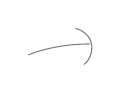
\begin{tikzpicture}\draw[gray] (0,0) .. controls (.24,.10) and (.54,.14) .. (.78,.14); \draw[gray] (.60,.34) .. controls (.89,.25) and (.83,-.03) .. (.71,-.12);\end{tikzpicture}}

Et la commutativité de (1) signifie la commutativité de (2) \uline{pour les objets}. Mais bien sûr on la veut aussi pour les flèches, i.e. on veut la commutativité du diagramme. $*$

% slanted
\margin{Donner l'exemple des morphismes de dérivateurs, définis par \unsure{des} foncteurs \tikz[baseline=(m.base)]\node[draw=gray,ellipse,inner sep=1pt] (m) {\unsure{sur|entre}}; des Cat. de modèles $(\unsure{\mathcal M|\mathscr M},\Sigma)\unsure{\longrightarrow|-}(\mathcal M',\Sigma')$}

Sans doute on veut un peu plus sur les morphismes de dérivateurs -- on veut une commutation aux $f_{*}$ et \inserted{(?)} aux $f_{!}$ (cette fois seulement iso. can. près) \ldots

% slanted
\margin{Commutation \unsure{à|:} \unsure{$f_{*}$ (resp. à $f_{!}$)} : morphisme \uline{exact à g.} (resp. à droite), les morphismes \uline{\unsure{exacts|existent}} sont \unsure{ceux} à la fois exacts \unsure{à g.} et à \unsure{dr.}}

% archive sheet number: 16
